\chapter{How He Built a \$200 Million-per-Year Security Company}

The interview opens with the visible result: luxury cars, a large Los Angeles house, and the question that turns display into investigation. We are not trying to explain wealth by pointing back at wealth. We are trying to reconstruct the operating chain behind it: early pressure, a home-security business, a later solar expansion, the cash rules that kept risk from becoming fragility, and the repeated habit of turning a dream into dates, quotas, and action.

\section{The Visible Puzzle and the Pressure Source}

The first beat is intentionally concrete. The narrator points to the Lamborghinis, the Aston Martin, and the house, then asks what Edwin Arroyave did to put himself there. That is the right order for the notes as well. The visible object is the puzzle; the answer has to be built.

The transcript immediately moves backward. Edwin says he was born in Colombia, came to the United States at six, and grew up in poverty. Both parents ended up in jail. When his father was put away for a long time, Edwin promised that he would take care of the house, and he describes becoming head of household at fifteen.

That early pressure is not yet a business model, but it is already a constraint. Later, when he talks about urgency, necessity, pressure situations, and survival, those ideas are not floating abstractions. They are rooted in the first condition of the story:

\begin{equation}
\text{early pressure}
=
\text{family responsibility}
-
\text{ordinary readiness}.
\end{equation}

This is not an accounting identity. It is a compact way of preserving the opening logic: before there is scale, there is a person forced to act before he feels fully prepared.

\section{The Business Base: Security, Solar, and Scale}

The interview then moves from origin story to operating facts. Edwin identifies the industry as home security. He says he has been in that business for twenty-five years, started his first business at twenty-one, and is forty-six at the time of the conversation. The timeline is simple:

\begin{equation}
46-21=25\text{ years}.
\end{equation}

The revenue claims are just as direct. The business has generated more than \$600 million over the career, and he says the largest single year will be the current one, at about \$200 million:

\begin{align}
R_{\text{career}} &> \$600{,}000{,}000,\\
R_{\text{year}} &\approx \$200{,}000{,}000.
\end{align}

Here \(R\) means revenue. The transcript does not give profit, valuation, tax treatment, ownership percentage, or net worth. The careful claim is that the business generated these amounts.

Once those numbers are on the table, the interviewer asks the natural scale question: many people have ideas, but how does one grow a business into nine figures? Edwin's first answer is influence. To bring in good people, they have to believe in the leader. Good people have options; therefore the leader's dream has to be large enough that their dreams can fit inside it.

A cautious operating dependency is:

\begin{equation}
\text{scale}
\;\Longleftarrow\;
\text{recruiting belief}
+
\text{credible dream}
+
\text{first action}.
\end{equation}

The last term is essential. Edwin does not let the answer stay in the language of vision. He moves immediately to acting before the resources are complete.

\subsection{Question \& Answer}

\paragraph{Question.}
How can acting before we have what we need be rational rather than merely reckless?

\paragraph{Answer.}
The answer is the minivan story. Edwin says that when he started the home-security company, he bought the minivan before he had the people. The sales model required teams going door to door in vans. He did not yet have the full team, but he put money behind the future he intended to build.

The mechanism is not blind spending. It is commitment under uncertainty. Once the resource is purchased, the future becomes less optional. Edwin calls the resulting pressure a necessity level: a sudden willingness that unlocks ability he did not know he had. In his phrasing, low stress is low performance; uncomfortable situations can raise the urgency level enough to change behavior.

\begin{figure}
\centering
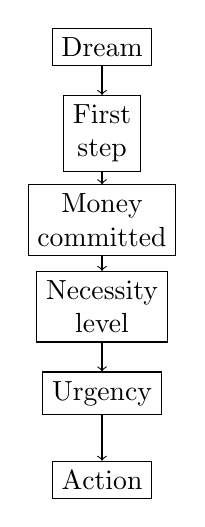
\begin{tikzpicture}[x=1cm,y=1cm]
\node[draw, align=center] (a) at (0,0) {Dream};
\node[draw, align=center] (b) at (0,-1.10) {First\\step};
\node[draw, align=center] (c) at (0,-2.20) {Money\\committed};
\node[draw, align=center] (d) at (0,-3.30) {Necessity\\level};
\node[draw, align=center] (e) at (0,-4.40) {Urgency};
\node[draw, align=center] (f) at (0,-5.50) {Action};
\draw[->] (a) -- (b);
\draw[->] (b) -- (c);
\draw[->] (c) -- (d);
\draw[->] (d) -- (e);
\draw[->] (e) -- (f);
\end{tikzpicture}
\caption{A transcript-grounded reconstruction of Edwin's commitment sequence. The resource is committed before the team is complete, creating necessity and urgency.}
\end{figure}

This is still a bounded claim. The minivan works in the story because it is attached to a known sales process. The uncertain part is the timing of the people; the operating path itself is not imaginary.

\section{Focus First, Diversify Later}

The next question raises a familiar entrepreneurial fork: diversify across industries, or focus on one thing? Edwin answers by sequence rather than slogan. First, focus on one thing. Become good enough that the business becomes the bread and butter. Then diversify from a base of cash flow and earned skill.

The numerical comparison is the key evidence. It took seventeen years to do \$40 million in one year in security. It took one year to do that in solar:

\begin{align}
R_{\text{security}} &= \$40{,}000{,}000
\quad \text{after }17\text{ years},\\
R_{\text{solar}} &= \$40{,}000{,}000
\quad \text{after }1\text{ year}.
\end{align}

The transcript does not prove a universal scaling law. It gives a transfer claim. Sales discipline, recruiting skill, standards, pressure tolerance, and cash-flow judgment were built in the first business and then carried into the second. A cautious form is:

\begin{equation}
\text{new-business speed}
\approx
\text{market opportunity}
+
\text{transferred operating discipline}.
\end{equation}

The word ``transferred'' does the work. Solar did not start from nothing; it started after seventeen years of paying the price in security.

\section{Cash Rules and the Reserve Account}

The discussion then moves from revenue to financial advice. Edwin says he did not really have a mentor early on, so he had to figure things out. One rule mattered: he split his check three ways. He lived on a third, put one third toward IRS and savings, and put the other third into a reserve account that no one could touch.

Let \(I\) be a check or income event. The spoken rule can be reconstructed as:

\begin{align}
I_{\text{living}} &\approx \frac{1}{3}I,\\
I_{\text{IRS+savings}} &\approx \frac{1}{3}I,\\
I_{\text{reserve}} &\approx \frac{1}{3}I,
\end{align}

so that

\begin{equation}
I
\approx
I_{\text{living}}
+
I_{\text{IRS+savings}}
+
I_{\text{reserve}}.
\end{equation}

The notation is deliberately modest. It is not a tax model, and it is not a legal structure. The transcript gives a behavioral structure: ordinary spending is constrained, obligations are funded, and a reserve exists precisely because hard times are expected.

\begin{table}
\centering
\begin{tabular}{|c|c|c|}
\hline
Living & IRS + savings & Reserve \\
\hline
Spendable third & Obligations & Untouchable buffer \\
\hline
\end{tabular}
\caption{The three-way check split, reconstructed from Edwin's financial advice.}
\end{table}

The reserve account is not just thrift. It is a survival design. Edwin says that if someone asked him for money, that reserve account did not exist. That fiction made the reserve real. It protected the business builder from confusing access with availability.

\section{A Dream Converted Into a Weekly Sales Requirement}

The strongest arithmetic in the interview comes from the story of buying his mother a house. Edwin says he promised his mother that he would buy her a dream house. At an open house, the dream became numerical: \$12,000 for the down payment and \$1,400 per month.

He then made the claim concrete: the home would be hers in ninety days. The target can be written as:

\begin{equation}
D=\$12{,}000,
\qquad
M=\$1{,}400/\text{month},
\qquad
T=90\text{ days}.
\end{equation}

The transcript then gives the operating breakdown. Ninety days is roughly twelve weeks, and Edwin says he needed eight to ten sales for twelve weeks straight:

\begin{align}
90\text{ days} &\approx 12\text{ weeks},\\
S_{\text{week}} &= 8\text{--}10\text{ sales/week}.
\end{align}

\paragraph{Worked target decomposition.}
The point is not to infer a commission per sale. The transcript does not supply one. The useful derivation is the conversion of an emotional promise into a repeated operating requirement:

\begin{enumerate}
\item State the promise: buy the house for his mother.
\item Put a date on it: \(T=90\) days.
\item Convert the time window into selling periods: \(90\text{ days}\approx 12\text{ weeks}\).
\item Identify the weekly sales target: \(S_{\text{week}}=8\text{--}10\).
\item Let the weekly target govern the day: do not stop merely because the day is late and the result has not appeared.
\end{enumerate}

\begin{figure}
\centering
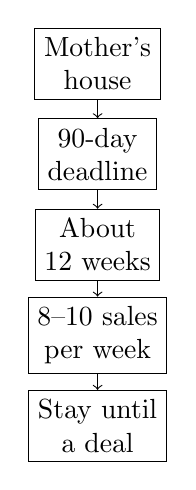
\begin{tikzpicture}[x=1cm,y=1cm]
\node[draw, align=center] (p) at (0,0) {Mother's\\house};
\node[draw, align=center] (d) at (0,-1.15) {90-day\\deadline};
\node[draw, align=center] (w) at (0,-2.30) {About\\12 weeks};
\node[draw, align=center] (s) at (0,-3.45) {8--10 sales\\per week};
\node[draw, align=center] (n) at (0,-4.60) {Stay until\\a deal};
\draw[->] (p) -- (d);
\draw[->] (d) -- (w);
\draw[->] (w) -- (s);
\draw[->] (s) -- (n);
\end{tikzpicture}
\caption{A dream becomes operational when it is converted into a deadline and then into a weekly sales requirement.}
\end{figure}

This is the interview's clearest example of commercial arithmetic. The promise changes the meaning of a weak day. Without a dated target, quitting late in the day is easy to rationalize. With the target, the day remains unfinished until the required effort has been made.

It also explains Edwin's later comment about belief. He says he stopped looking desperate because he knew that somehow he would get a sale by the end of the day. In the transcript, belief is not detached from action. It is produced by repeated late effort that eventually yields results.

\section{The Abundance Formula}

After the sponsor interruption, the interview returns to money. The question is what separates the middle class from the wealthy. Edwin's answer is not initially about instruments or asset classes. It is about a relationship with money.

If a person is always worried about not having enough, he says, the person starts to hoard. If the person hoards everything, the person never goes out to touch or taste the dream. If the dream is never touched, the desire to act weakens. In that sequence, waiting for enough money becomes a trap:

\begin{equation}
\text{wait to have}
\;\Longrightarrow\;
\text{delay action}
\;\Longrightarrow\;
\text{remain stuck}.
\end{equation}

Edwin reverses the order. His abundance sequence is:

\begin{equation}
\text{become}
\;\Longrightarrow\;
\text{act}
\;\Longrightarrow\;
\text{have}.
\end{equation}

\subsection{Question \& Answer}

\paragraph{Question.}
Should a person wait until enough money is saved before taking the action that would change the situation?

\paragraph{Answer.}
In Edwin's telling, waiting can become a closed loop: worry, hoard, postpone, get hit by life, lose the cushion, and begin again. The alternative is to become first. Becoming means hope, faith, belief, and a sense of worth before the result is visible. Then comes action before all resources are present.

The next step is not vague optimism. It is breakdown. Once a person acts, Edwin says, a blueprint appears. The goal must be broken down until it becomes attainable; once attainable, it becomes realistic; once realistic, action becomes easier.

\begin{figure}
\centering
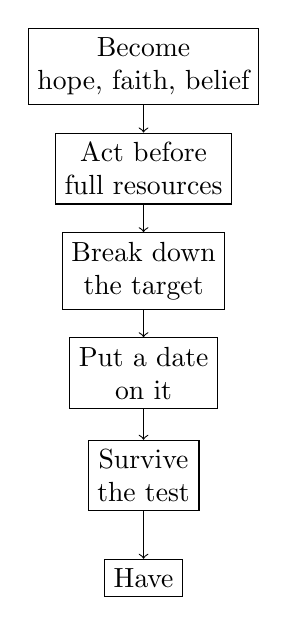
\begin{tikzpicture}[x=1cm,y=1cm]
\node[draw, align=center] (b) at (0,0) {Become\\hope, faith, belief};
\node[draw, align=center] (a) at (0,-1.30) {Act before\\full resources};
\node[draw, align=center] (bp) at (0,-2.60) {Break down\\the target};
\node[draw, align=center] (date) at (0,-3.90) {Put a date\\on it};
\node[draw, align=center] (test) at (0,-5.20) {Survive\\the test};
\node[draw, align=center] (h) at (0,-6.50) {Have};
\draw[->] (b) -- (a);
\draw[->] (a) -- (bp);
\draw[->] (bp) -- (date);
\draw[->] (date) -- (test);
\draw[->] (test) -- (h);
\end{tikzpicture}
\caption{The abundance formula as a process rather than an equation: becoming precedes action, and action produces a usable blueprint.}
\end{figure}

The hardest part, Edwin says, comes near the blessing. A test arrives. The person is knocked down and must choose whether to revert to the older self or continue forward, focus on what can be controlled, and trust that the right people will appear. The transcript is garbled in this region, but the structure is plain: the test is where the old identity tries to reclaim the decision.

\section{Faith, Happiness, and the Attention Filter}

The final movement broadens from business mechanics to the inner machinery that Edwin believes made those mechanics possible. The interviewer asks what advice he would give to someone without belief in God or faith. Edwin answers that, whether one likes it or not, one is faith-based. Faith and fear are both projections into a future that has not yet happened:

\begin{equation}
\text{faith}
=
\text{positive projection of the future},
\qquad
\text{fear}
=
\text{negative projection of the future}.
\end{equation}

This is Edwin's formulation. We should not turn it into a theorem of psychology. Its role in the interview is to explain why the imagined future matters: the person is already projecting something, and that projection governs present action.

The next distinction is between pleasure and happiness. Edwin says exterior factors such as exotic cars and large houses brought pleasure, but not stable happiness. Pleasure is a sensation and therefore unstable; in his words, it is balanced by the discomfort and pain one has to go through. His proposed alternative is living inside out rather than exterior in: gratitude exercises and the ability to turn a negative into a positive.

The last framework is the reticular activating system. Edwin describes it as part of the subconscious mind, filtering what reaches conscious attention. We should preserve the claim as his explanatory model, not expand it into neuroscience beyond the transcript. In his model, the filter passes signals connected to dreams, self-worth, and survival.

\begin{figure}
\centering
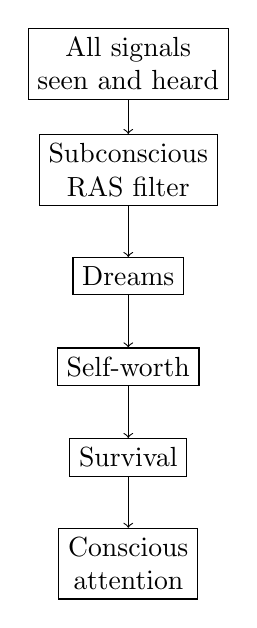
\begin{tikzpicture}[x=1cm,y=1cm]
\node[draw, align=center] (input) at (0,0) {All signals\\seen and heard};
\node[draw, align=center] (filter) at (0,-1.35) {Subconscious\\RAS filter};
\node[draw, align=center] (dream) at (0,-2.70) {Dreams};
\node[draw, align=center] (worth) at (0,-3.85) {Self-worth};
\node[draw, align=center] (survival) at (0,-5.00) {Survival};
\node[draw, align=center] (attention) at (0,-6.35) {Conscious\\attention};
\draw[->] (input) -- (filter);
\draw[->] (filter) -- (dream);
\draw[->] (dream) -- (worth);
\draw[->] (worth) -- (survival);
\draw[->] (survival) -- (attention);
\end{tikzpicture}
\caption{A narrow reconstruction of Edwin's attention-filter model. Dreams, self-worth, and survival are the categories he says make opportunities visible.}
\end{figure}

He then uses that model to reinterpret his own earlier decisions. At twelve, he daydreamed about making \$100,000 by twenty-one. He went to Beverly Hills and imagined ending up there. He had some self-worth from early accomplishments, and he needed success for survival because of promises to his parents. In the logic of the interview, those three filters made an opportunity visible when others thought leaving a \$70,000-a-year job was crazy.

\section{Summary}

The chapter's chain is concrete. Visible wealth raises the question, but the answer is not the wealth itself. Early pressure builds tolerance for urgency. A focused home-security business creates operating discipline. Influence recruits people. Commitment before complete resources creates necessity. The check is split so risk does not consume the whole system. A promise to buy a house becomes a 90-day target, then a weekly sales requirement. The abundance formula reverses the passive sequence of waiting to have enough and replaces it with becoming, acting, and then having.

The quantitative payload is modest but important: twenty-five years from first business to the interview, more than \$600 million in business revenue, a projected \$200 million year, a seventeen-year path to \$40 million in security, a one-year path to the same annual level in solar, an approximate three-way check split, and a 90-day house promise translated into eight to ten sales per week for twelve weeks. The numbers should remain attached to the stories that produced them, because here the arithmetic is the mechanism by which a dream becomes operational.